\section{Exascale Ray Tracing}
\label{sec:raytracing}

When designing our ray tracing prototype for exascale we focused on
two key aspects: (a) producing a task based application with (b) an
emphasis on avoiding communication. For simplicity, we consider here
only ray tracing scenes without reflection or refraction, although our
proposed algorithm can be extended to handle either in the future. Our
algorithm uses a simple voxel decomposition to split the work required
to trace a scene (which we will henceforth refer to as a ``domain'').

Primary camera rays are then sent into the system and propagate
through the domain. As secondary rays introduce most of the uncertainty
in the amount of communication necessary in a ray tracing algorithm,
we introduce a pre-processing technique that distributes light
information to each voxel prior to tracing the domain. This allows the
ray tracing step within each voxel to be completely independent of the
data in the rest of the domain. Using this algorithm we can predict an
upper bound on the amount of communication necessary (a domain that
contains no data), and extrapolate from there rough estimates on how
our algorithm might perform on an exascale system.

\subsection{Implementation}

We chose to implement our ray tracer using Intel’s implementation of
CnC, which is built on top of their Thread Building Blocks (TBB)
library. This runs on today’s multicore systems but has the potential
to do so on anticipated exascale systems.

Figure \ref{fig:cnc} shows the graph for our distributed ray tracer.
It shows data collections, step collections, and the dependencies
between them. The tags corresponding to each collection are also
shown. The control collection for the proposed model is static for all
steps and defined in an initialization step. The graph begins
execution when the object, lights, and camera data are provided, and
terminates when it produces an image.

Let us consider the parts of the graph individually.

\subsection{Tags}

The tags are different for many of the data and step collections but
share common elements. The FRAME tag refers to one specific frame in
the case of an animation. The INSTANCE tag refers to the current
iteration. The I, J, and K tags are iterators over 3D spatial data,
selecting a specific voxel. The RAY\_STEP tag allows for multiple
traversals of the same voxel in the same frame for secondary rays.

\subsection{Data Collections}
\label{sec:datacollections}

The OBJECT data collection contains input data for the domain from the
environment. Currently, this data is extracted from WaveFront
``\texttt{.obj}'' files. The DECOMPOSE\_DOMAIN step collection
partitions this data into voxels, producing the VOXEL\_OBJECT data
collection. Objects that span multiple voxels are duplicated. The
LIGHTS data collection contains data pertaining to light sources. The
VOXEL\_LIGHT data collection contains the same information as LIGHTS
plus a traced light mesh for each wall of a voxel. The CAMERA data
collection contains the location and direction of the camera. The
RAY\_PACKET data collection contains all the rays that intersect a
voxel wall for a given wall and iteration. The IMAGE data collection
contains the final image data.

\subsection{Step Collections}

Recall that these are where the computation is done. They may be
implemented in any programming language CnC supports, which is most of
them.

\subsubsection{DECOMPOSE\_DOMAIN}

As mentions in Section~\ref{sec:datacollections} the DECOMPOSE\_DOMAIN
step takes the data to be traced as input and produces subsets of that
data based on voxel decomposition. As load balancing is not a concern,
a uniformly-gridded voxel decomposition is sufficient. The number of
voxels produced is set at runtime and should be more than the number
of nodes available.
% RRL: Is this really a constraint?

\subsubsection{DISTRIBUTE\_LIGHTS}

In order to reduce the communication of secondary rays,
the DISTRIBUTE\_LIGHTS step is responsible for distributing light
information to each voxel. This guarantees each voxel will only need
to communicate with its direct neighbors. The light information
produced for each voxel contains the original light sources as well as
a light source mesh for each light and each wall of the voxel. The
mesh is produced by tracing rays from each light source to uniformly
spaced points along a voxel wall, see Figure \ref{fig:light}. Where
the rays intersect the wall, new point or directional light sources
are created. If the ray is blocked, the node in the light mesh is
tagged as in shadow.

\begin{figure}[!htb]
\centering
\begin{subfigure}{.49\columnwidth}
 \centering
  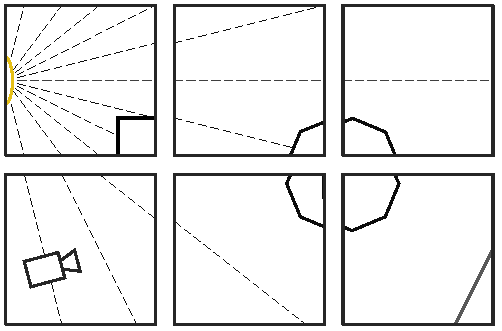
\includegraphics[width=.98\columnwidth]{drawings/Lights1.pdf}
  \caption{Initial light rays}
\end{subfigure}
\begin{subfigure}{.49\columnwidth}
 \centering
  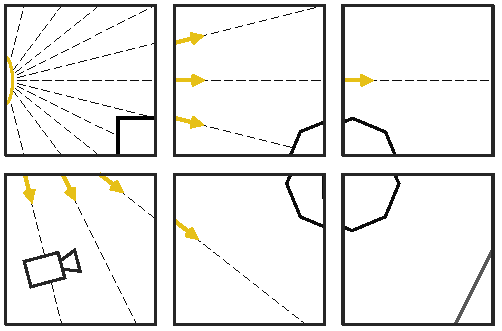
\includegraphics[width=.98\columnwidth]{drawings/Lights2.pdf}
  \caption{Point light sources}
\end{subfigure}
\caption{Light Ray Distribution}
\label{fig:light}
\end{figure}

\subsubsection{DISTRIBUTE\_RAYS}

The DISTRIBUTE\_RAYS step is responsible for sending each voxel its
first iteration of ray information. This is an empty set of data for
all voxels except the voxel containing the camera if the camera is
positioned within the domain. If the camera is outside the domain
(e.g. in an orthographic view), multiple voxels may be initialized.

\subsubsection{TRACE\_VOXEL}

The TRACE\_VOXEL step is the heart of the application. This step
executes multiple times for each voxel, depending on the size of the
domain. Each time TRACE\_VOXEL executes, it consumes ray packets from
each of its neighbors. It then traces the rays over its subset of the
domain. If a ray intersects with an object, secondary rays from each
light source are considered if the corresponding point or directional
light source from the voxels light mesh is not in shadow.

Rays that do not intersect objects within the voxels and reach the
voxels walls are collected and passed to the corresponding neighbor on
the next iteration. See Figure~\ref{fig:trace}. Because we are not
considering reflection or refraction, we know the maximum amount of
times we will have to communicate a single ray across voxel borders in
the worst case is proportional to domain size. This allows us to
prescribe the a maximum number of instances of TRACE\_VOXEL in an
initialization step. For the example in Figure~\ref{fig:trace}, that
maximum is 3. As each step will eventually be executed on a single
node of a cluster we plan to implement TRACE\_VOXEL using Embree,
Intel’s ray tracing kernel, in order to optimize per node performance.

\begin{figure}[!htb]
\centering
\begin{subfigure}{.49\columnwidth}
 \centering
  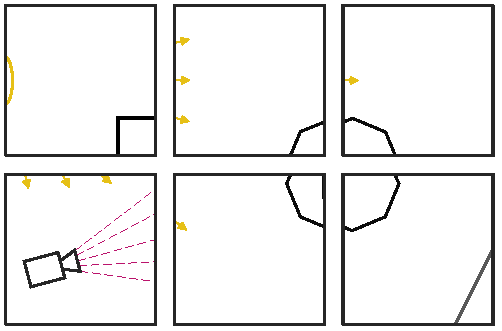
\includegraphics[width=.98\columnwidth]{drawings/Trace1.pdf}
  \caption{Distribute rays}
\end{subfigure}
\begin{subfigure}{.49\columnwidth}
 \centering
  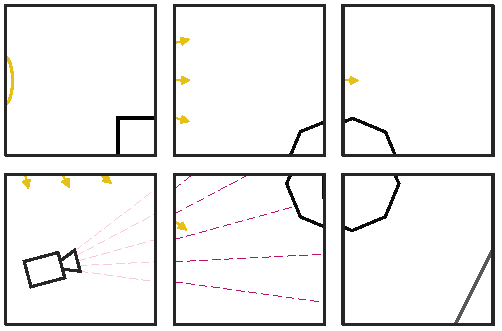
\includegraphics[width=.98\columnwidth]{drawings/Trace2.pdf}
  \caption{Trace voxel; ray step 1}
\end{subfigure}
\begin{subfigure}{.49\columnwidth}
 \centering
  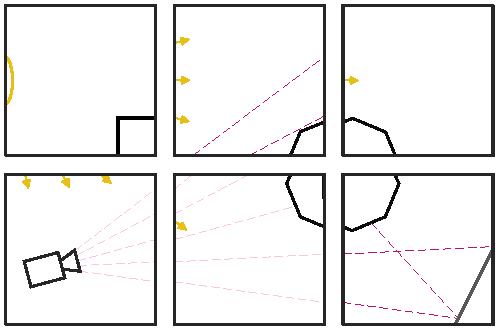
\includegraphics[width=.98\columnwidth]{drawings/Trace3.pdf}
  \caption{Trace voxel; ray step 2}
\end{subfigure}
\begin{subfigure}{.49\columnwidth}
 \centering
  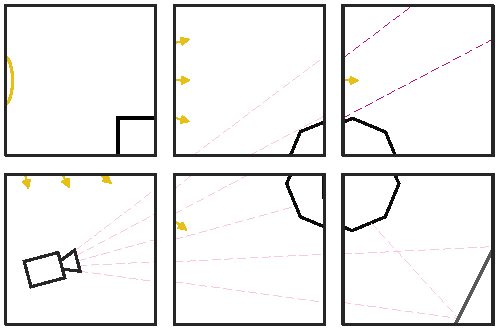
\includegraphics[width=.98\columnwidth]{drawings/Trace4.pdf}
  \caption{Trace voxel; ray step 3}
\end{subfigure}
\caption{Trace Voxel}
\label{fig:trace}
\end{figure}

\subsubsection{PRODUCE\_IMAGE}
When all steps in TRACE\_VOXEL have completed, the final set of ray
packets is produced. Each ray in that packet contains the information
that may be necessary to produce the final image. Merging these is the
responsibility of the PRODUCE\_IMAGE step.

\subsection{Textual CnC Graph File}
To give a more concrete example of how the CnC graph file is
implemented, we include a simplified version of the textual
representation of TRACE\_VOXEL in Figure~\ref{fig:tracevoxel}. In
addition to the step declaration, the code includes the SCENE and
RAY\_PACKET data collections as well as the control dependencies from
the environment for TRACE\_VOXEL.

% Code..
\begin{figure*}[t!]
  \begin{center}
    
\begin{lstlisting}[basicstyle=\ttfamily]
/******************************************************************************
//* Item collection declarations */

// data for each voxel, produced by decompose_domain
[ voxel_object *voxel : frame, i, j, k ];

// ray data passed to neighbors, produced by camera and trace_voxel
[ ray_packet *rays : frame, ray_step, neighbor, i, j, k ];

/******************************************************************************
//* CnC steps */

( trace_voxel : frame, ray_step, i, j, k )
<- [ voxel: frame, i, j, k],
   [ rays : frame, ray_step  , 0, i  , j  , k   ] $when(i<#voxels_i-1),
   [ rays : frame, ray_step  , 1, i  , j  , k   ] $when(i>0),
   [ rays : frame, ray_step  , 2, i  , j  , k   ] $when(j<#voxels_j-1),
   [ rays : frame, ray_step  , 3, i  , j  , k   ] $when(j>0),
   [ rays : frame, ray_step  , 4, i  , j  , k   ] $when(k<#voxels_k-1),
   [ rays : frame, ray_step  , 5, i  , j  , k   ] $when(k>0)
-> [ rays : frame, ray_step+1, 0, i-1, j  , k   ] $when(i>0),
   [ rays : frame, ray_step+1, 1, i+1, j  , k   ] $when(i<#voxels_i-1),
   [ rays : frame, ray_step+1, 2, i  , j-1, k   ] $when(j>0),
   [ rays : frame, ray_step+1, 3, i  , j+1, k   ] $when(j<#voxels_j-1),
   [ rays : frame, ray_step+1, 4, i  , j  , k-1 ] $when(k>0),
   [ rays : frame, ray_step+1, 5, i  , j  , k+1 ] $when(k<#voxels_k-1);

/******************************************************************************
//* Input output relationships from environment */

( $initialize: () )
-> (trace_voxel : $range(0, #num_frames), $range(0, #ray_steps),
           $range(0, #voxels_i), $range(0, #voxels_j), $range(0, #voxels_k));

\end{lstlisting} 
  \end{center}
  
  \caption{The TRACE\_VOXEL Section of the CnC Graph File. This has
    been somewhat simplified for readability.}
  \label{fig:tracevoxel}
\end{figure*}

Under the \emph{Item collection declaration} section we see two item
collections being declared. Once for the domain and one for the ray
packets. Instances of the domain indexed using frame, i, j, and k
which correspond to the frame in the case of an animation and the
3-dimensional identifier for a given voxel. Ray packets are indexed
similarly but also include an entry for the current ray step as well
as a neighbor identifier.

Under \emph{CnC steps} we see the declaration for TRACE\_VOXEL. Each
TRACE\_VOXEL step is indexed using the frame, the voxels i, j, k and
the current ray step. The specific instances of the domain and ray
data consumed and produced by TRACE\_VOXEL can be declared using the
RAY\_STEP tag. The step will always consume its scene data. It may
then consume an incoming ray packet and/or produce an outgoing ray
packet for each of the voxel's interior walls.

Under \emph{Input output relationships from environment} we see the
control for TRACE\_VOXEL. In the initialize step we will produce an
instance of TRACE\_VOXEL for every frame in our animation, for every
step in our ray steps, and for each voxel in our scene's
decomposition.

%%% Local Variables: 
%%% mode: latex
%%% TeX-master: "main"
%%% End: 
